\documentclass[10pt, conference, compsocconf]{IEEEtran}
\usepackage{graphicx}
\usepackage{subcaption}
\usepackage{float}
\usepackage{amsmath}
\usepackage{hyperref}
\usepackage{booktabs}
\usepackage{booktabs} % For better horizontal rules
\usepackage{siunitx}  % For aligning numbers by decimal point
\hypersetup{
	colorlinks=true,
	linkcolor=black,
	filecolor=magenta,      
	urlcolor=cyan,
}


\title{Structure equation modeling}

\begin{document}
	
	
	\maketitle
	
	\section{Overview}	
	\begin{figure}[h!]
		\centering
		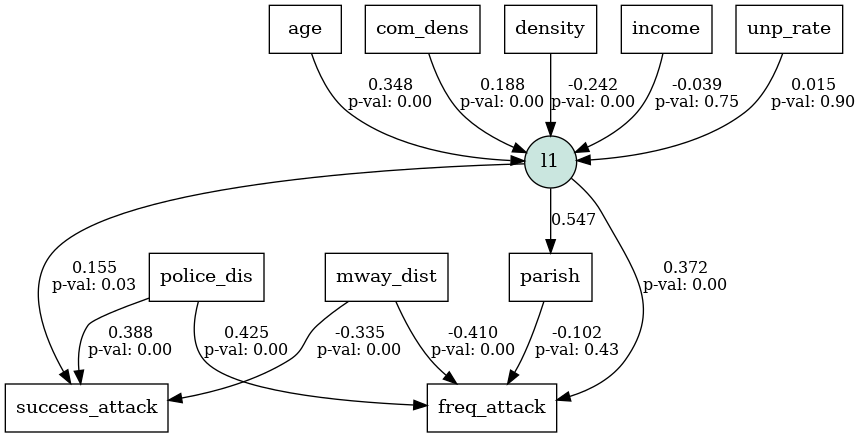
\includegraphics[width=\linewidth]{semresult2.png}
		\caption{SEM Model}
		\label{fig:Model}
	\end{figure}
	

	
	\begin{enumerate}
		\item Name of objective: Diagonally Weighted Least Squares 
		\item  Optimization method: SLSQP
		\item  Objective value: 0.058
		\item  Number of iterations: 51
	\end{enumerate}	
	\textbf{Equation used}
\begin{align}
	& l1 =\sim \text{parish} \\
	& \text{success\_attack} \sim l1 + \text{mway\_dist} + \text{police\_dis} \\
	& \text{freq\_attack} \sim l1 + \text{parish} + \text{mway\_dist} + \text{police\_dis} \\
	& l1 \sim \text{com\_dens} + \text{age} + \text{income} + \text{unp\_rate} + \text{density} 
\end{align}

	
	\begin{enumerate}
		\item DoF: 39
		\item chi2: 41.931951
		\item chi p-value: 0.344902
		\item CFI: 0.998558
		\item GFI: 0.979888
		\item RMSEA: 0.010204
	\end{enumerate}
	
	
		
	\begin{table}[htbp]
		\centering
		\caption{Parameter Estimates}
		\label{tab:parameter_estimates}
		\begin{tabular}{
				l
				l
				l
				S[table-format=2.6] % Adjust the number of digits before and after the decimal point as needed
				S[table-format=1.6] % Adjust the number of digits before and after the decimal point as needed
				S[table-format=2.6] % Adjust the number of digits before and after the decimal point as needed
			}
			\toprule
			Variables & {Estimate} & {Std. Err} & {z-value} \\
			\midrule
			parish $\longrightarrow$ L & 1.000000 & null & null \\
			L $\longrightarrow$ com\_dens & 0.035499 & 0.011404  & 3.112724 \\
			L $\longrightarrow$ age & 0.106035 & 0.020269  & 5.231404   \\
			L $\longrightarrow$ income & -0.009657 & 0.029956  & -0.322363  \\
			L $\longrightarrow$ unp\_rate & 0.008836 & 0.07163  & 0.123352\\
			L $\longrightarrow$ density & -0.075234   & 0.018266 & -4.118882    \\
			
			
			success\_attack $\longrightarrow$ L & 0.015101 & 0.007025 & 2.149691 \\
			
			success\_attack $\longrightarrow$ mway\_dist & -0.000104 & 0.000012 & -8.371719  \\
			success\_attack $\longrightarrow$ police\_dis & 0.000357 & 0.000031 & 11.462717 \\
			
			freq\_attack $\longrightarrow$ L & 0.054424 & 0.015723 & 3.461409 \\
			
			freq\_attack $\longrightarrow$ parish & -0.008179 & 0.010427 & -0.784397 \\
			freq\_attack $\longrightarrow$ mway\_dist & -0.000191  & 0.000018 & -10.629688    \\
			freq\_attack $\longrightarrow$ police\_dis & 0.000589 & 0.000045 & 13.055707 \\
			\bottomrule
		\end{tabular}
	\end{table}
	
	
	
	\newpage
	\section{Model Explanation}	
	
	\textbf{Magnitude of Coefficients:} The magnitudes of the coefficients indicate the strength and direction of the associations. A larger magnitude suggests a stronger association between the variables.
	
\subsection{Geographic}	
	It was already identified with scatter plot visualization that police distance and motorway distance share negative and positive linear association relationship respectively with frequency and success of attack.\\
	The SEM model sheds lights on the following statements: -
	\begin{enumerate}
		\item Positive association of police distance with success and frequency of attack indicates as the value of "police distance" increases, the success and frequency of attack tends to increase as well and vice versa.
		\item  Negative association of motorway distance with success and frequency of attack indicates as the value of motorway distance increases the success and frequency of attack decreases and vice versa.
	\end{enumerate}
\subsection{Demographic}
The demographic factors do not influence the success and frequency of attack directly , they influence it through a latent variable \textbf{L}. 
\textbf{L} is a latent variable measured using parish to see the influence of demographic factors  indirectly through \textbf{L}  on success and frequency of attack.\\
\textbf{Association with L}
\begin{enumerate}
	\item  Age and Commercial density share a positive association with \text{L}, which can be interpreted as increase in age rate and commercial density of an area leads to increase in the latent factor \textbf{L}. 
	\item Population density is associated negatively with \textbf{L} indicating with increase in population density the latent variable tends to decrease.
	\item Income and unemployment rate of the area have very low association in addition to that the P value (\textgreater0.05) of these factors indicate that they are not statistically significant. 
\end{enumerate}

\textbf{Association of L with success and frequency of attacks}
The latent variable \textbf{L} is measured using parish which is a categorical column ranging from 1 to 20 and each point represent a local neighborhood in Lisbon.

\begin{enumerate}
	\item L is positively associated with both frequency and success of attack with p value indicating that the association is statistically significant.
\end{enumerate}


\subsection{Conclusion}

Parish direct influence on frequency of attack is not statistically significant but the latent variable measured using parish which is predicted using demographic variables  shows a positive association with frequency and success of attack.

Increase in latent variable means with increase in \textbf{L}, the average age rate and commercial density of the area increase and population density decreases which overall lead to  increase in success and frequency of attack and vice versa.



Parishes direct influence on success of attack is not statistically significant (identified by adding parish in 2nd equation) as such that path was removed as it also caused the model behavior change (i.e. Introducing a CFI value greater then 1).

\section{Additional information}
As our dataset is biased with more values of non attacked ATMs then attacked ATMs,
The above model was run through a bias correction technique which resamples the mean of the data to adjust parameter estimates in statistical models to account for potential biases in the data or estimation procedure. This techniques aimed to improve the accuracy and reliability of parameter estimates by accounting for various sources of bias, such as sampling variability, measurement error, or model misspecification.\\
Resampling techniques involve repeatedly sampling from the data or model and recalculating parameter estimates to assess their variability and potential bias.

The number of resampling samples used in the bias correction process in n = 500.\\
For which the result obtained with resampling the mean and without resampling the mean were same.
The only difference in the bias corrected model is that it shows parish has a direct influence on frequency of attack.
\\
Bias correction can have a significant influence on the results of a structural equation model.
By accounting for biases in parameter estimates, bias correction techniques can lead to more accurate and reliable model estimates.
Bias correction helps to improve the validity and robustness of the conclusions drawn from the SEM analysis, enhancing confidence in the relationships and patterns identified in the data.
\\
Overall, with resampling and mean correction parameters helps to address potential biases in SEM parameter estimates, leading to more reliable and robust results. It is an important step in ensuring the validity and accuracy of SEM analyses, especially in situations where data quality or model assumptions may be uncertain.

\newpage
\textbf{Comparison of models}
\vspace{2cm}
\begin{figure}[H]
	
	\begin{subfigure}[b]{\linewidth}
		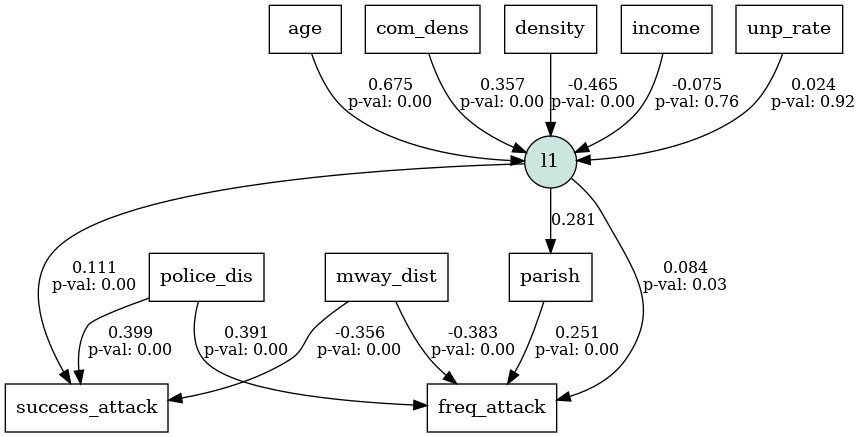
\includegraphics[height=0.2\textheight]{semresultbias.png}
		\caption{Bias Corrected Model}
		\label{bias}
	\end{subfigure}%

\vspace{2cm}

	\begin{subfigure}[b]{\linewidth}
		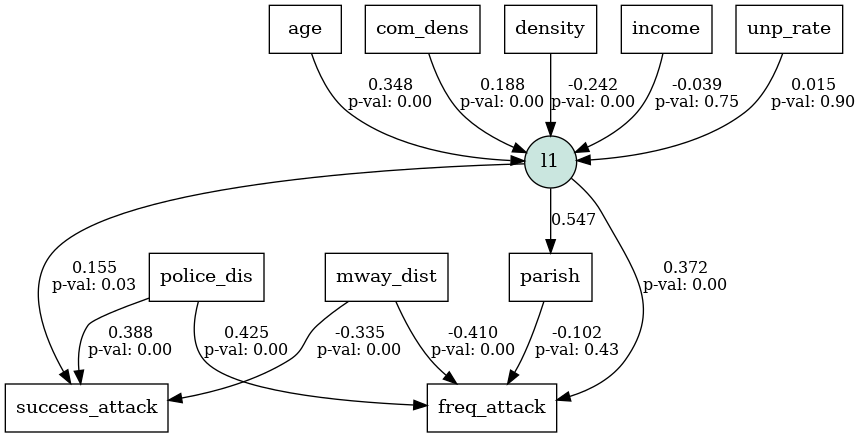
\includegraphics[height=0.2\textheight]{semresult2.png}
		\caption{Original Model}
		\label{fig:Model}
	\end{subfigure}

	\caption{Comparison of SEM Models}
	
\end{figure}
\end{document}